\begin{figure}[htbp]
\centering
\setlength{\tabcolsep}{1pt}
\begin{tabular}{cccc}
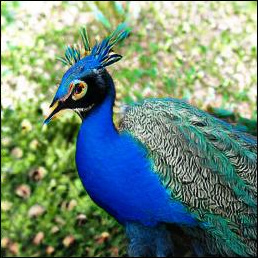
\includegraphics[width=0.24\textwidth]{images/samples0/Peacock0.jpg} & 
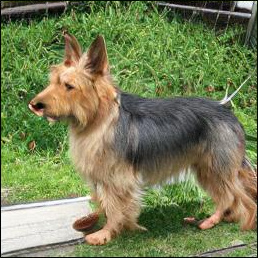
\includegraphics[width=0.24\textwidth]{images/samples0/dog0.jpg} &
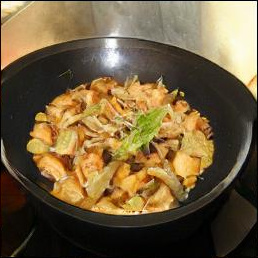
\includegraphics[width=0.24\textwidth]{images/samples0/wok0.jpg} & 
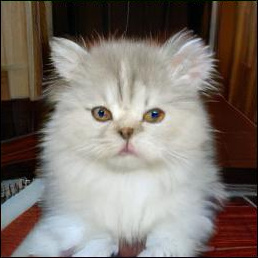
\includegraphics[width=0.24\textwidth]{images/samples0/Cat0.jpg} \\
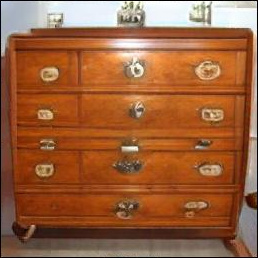
\includegraphics[width=0.24\textwidth]{images/samples0/dresser0.jpg} & 
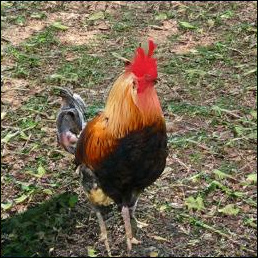
\includegraphics[width=0.24\textwidth]{images/samples0/bird3.jpg} &
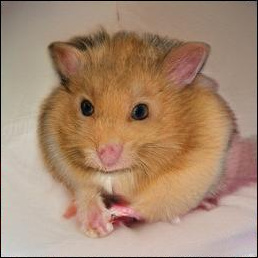
\includegraphics[width=0.24\textwidth]{images/samples1/256hamster0.jpg} & 
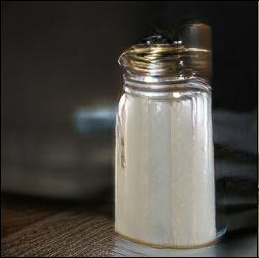
\includegraphics[width=0.24\textwidth]{images/samples1/256saltshaker0.jpg} \\
\end{tabular}
\caption{Samples generated by our BigGAN model at 256$\times$256 resolution.}
\label{appendix_samples256}
\end{figure}


\begin{figure}[htbp]
\centering
\setlength{\tabcolsep}{1pt}
\begin{tabular}{cccc}
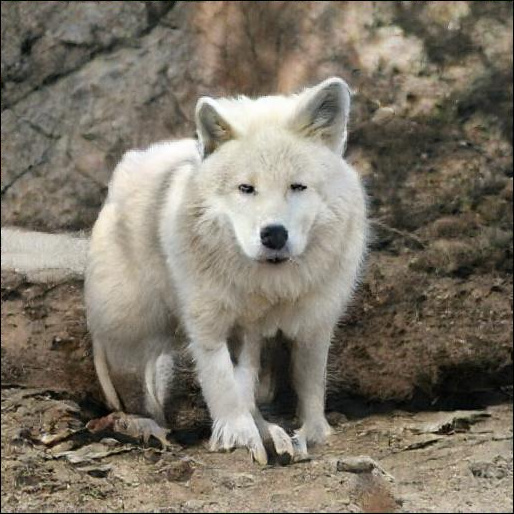
\includegraphics[width=0.24\textwidth]{images/samples1/512wolf0.jpg} & 
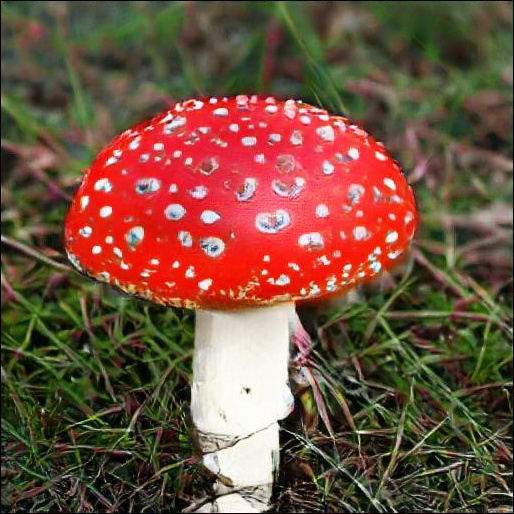
\includegraphics[width=0.24\textwidth]{images/samples1/512mushroom0.jpg} &
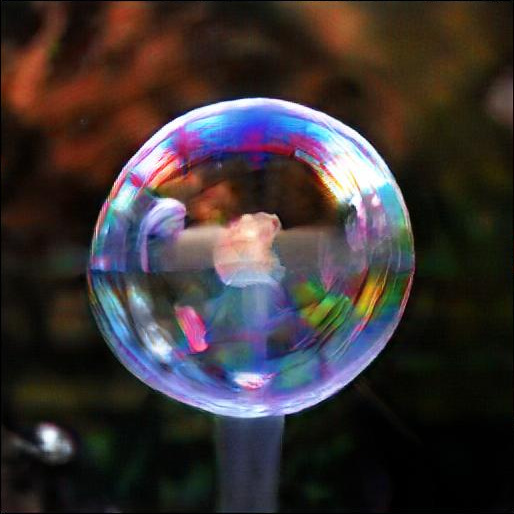
\includegraphics[width=0.24\textwidth]{images/samples1/512bubble0.jpg} & 
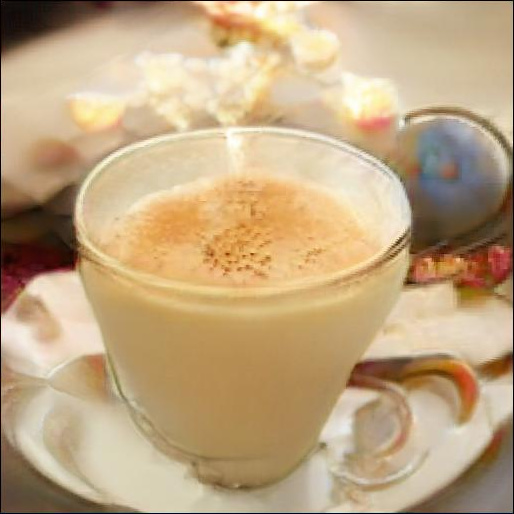
\includegraphics[width=0.24\textwidth]{images/samples1/mocha0.jpg} \\
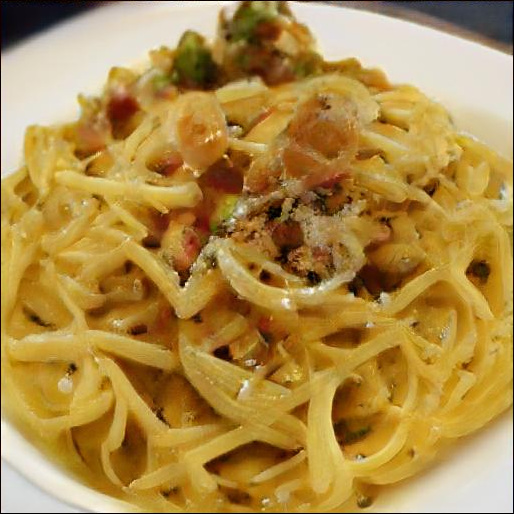
\includegraphics[width=0.24\textwidth]{images/samples1/512pasta0.jpg} & 
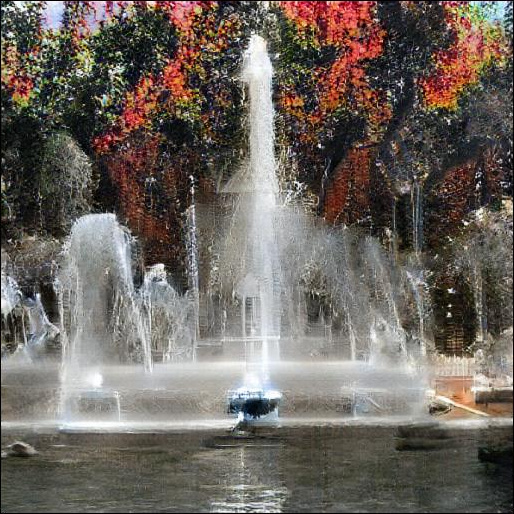
\includegraphics[width=0.24\textwidth]{images/samples1/512fountain0.jpg} &
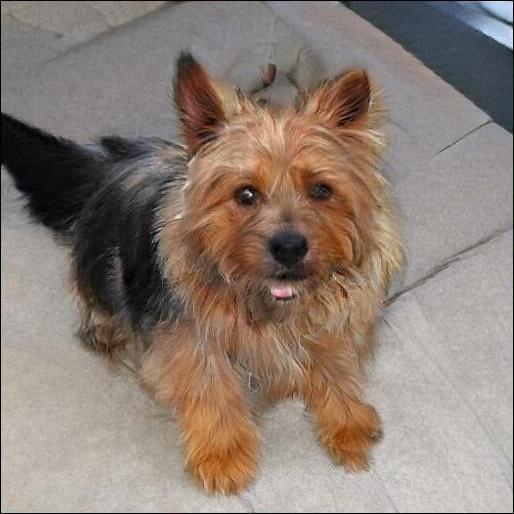
\includegraphics[width=0.24\textwidth]{images/samples1/512dog0.jpg} & 
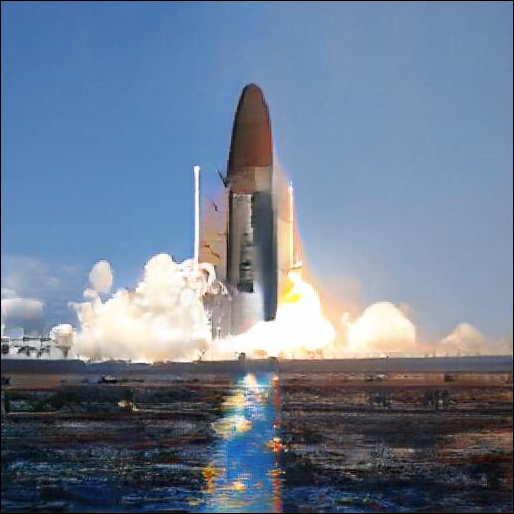
\includegraphics[width=0.24\textwidth]{images/samples1/512rocket0.jpg} 
\end{tabular}
\caption{Samples generated by our BigGAN model at 512$\times$512 resolution.}
\label{appendix_samples512}
\end{figure}

\begin{figure}[htbp]
\centering
\setlength{\tabcolsep}{1pt}
\begin{tabular}{cc}
\subf{\begin{tabular}{cc}
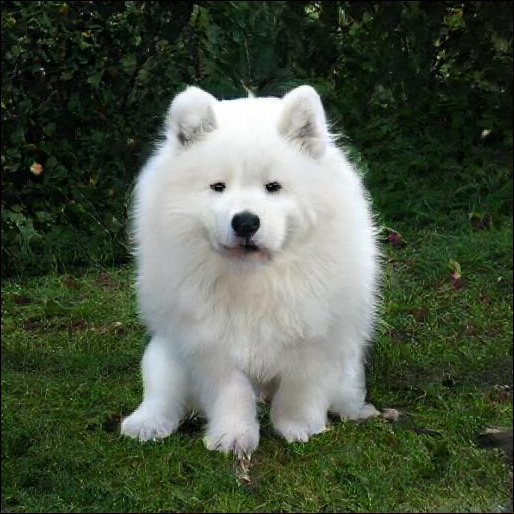
\includegraphics[width=0.24\textwidth]{images/samples1/512dog2.jpg} & 
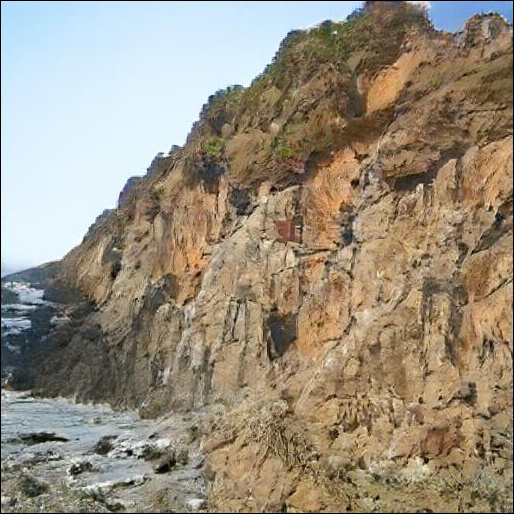
\includegraphics[width=0.24\textwidth]{images/samples1/512crags1.jpg} \\
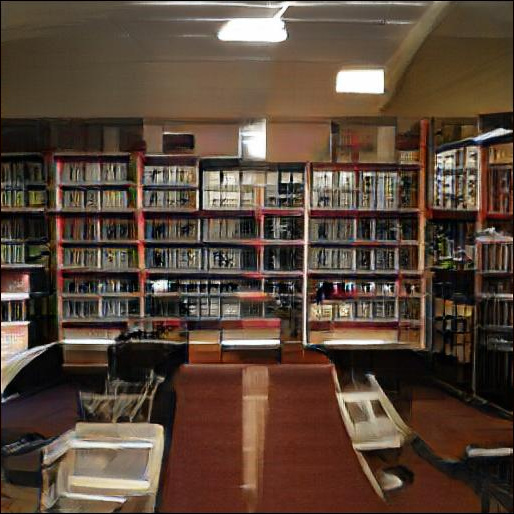
\includegraphics[width=0.24\textwidth]{images/samples1/512library0.jpg} & 
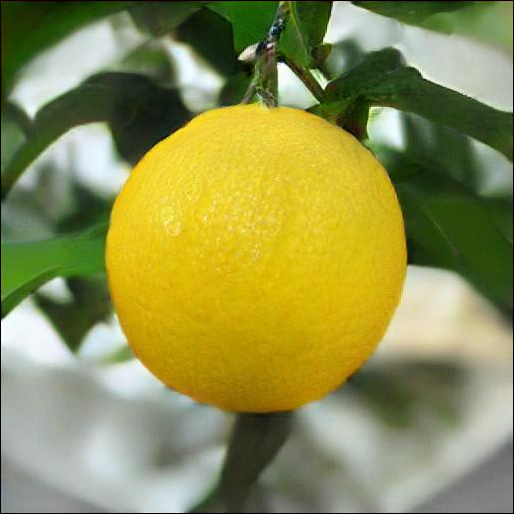
\includegraphics[width=0.24\textwidth]{images/samples1/512lemon0.jpg} 
\end{tabular}}{(a)} &
\subf{\begin{tabular}{cc}
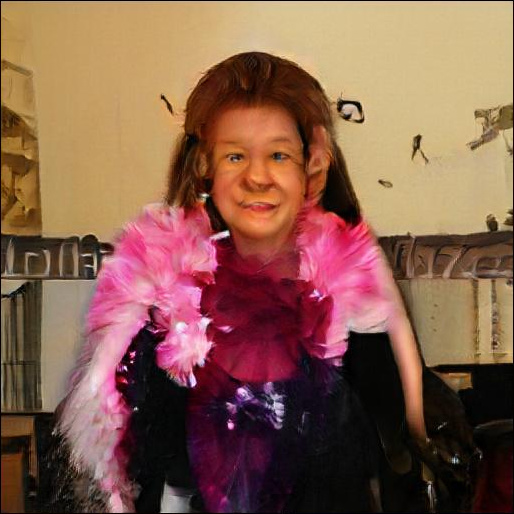
\includegraphics[width=0.24\textwidth]{images/samples1/featherboa0.jpg} & 
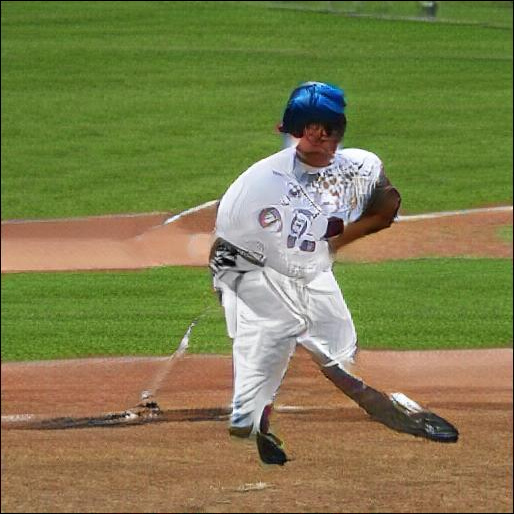
\includegraphics[width=0.24\textwidth]{images/samples1/512baseball0.jpg} \\
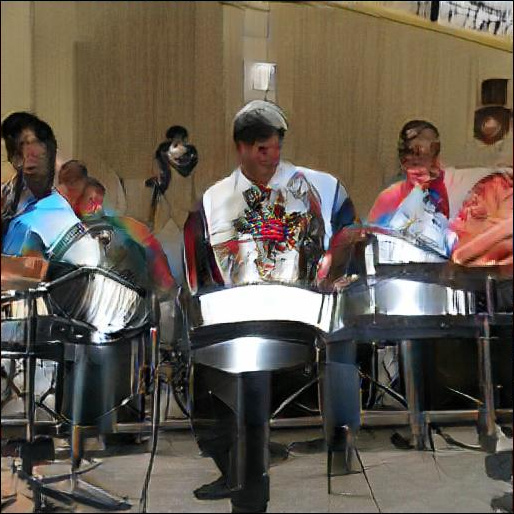
\includegraphics[width=0.24\textwidth]{images/samples1/512drummers0.jpg} & 
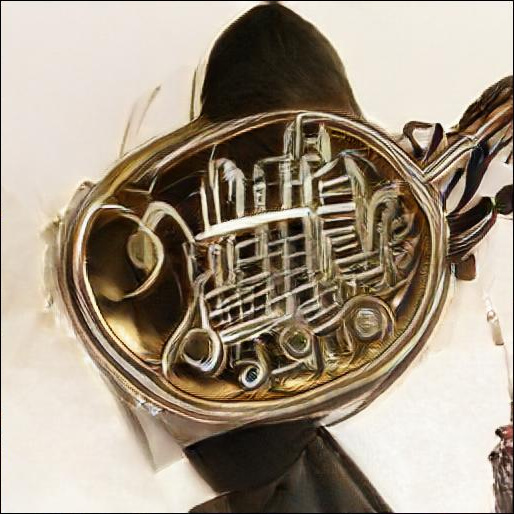
\includegraphics[width=0.24\textwidth]{images/samples1/512frenchhorn0.jpg}
\end{tabular}}{(b)}
\end{tabular}
\caption{Comparing easy classes (a) with difficult classes (b) at 512$\times$512. Classes such as dogs which are largely textural, and common in the dataset, are far easier to model than classes involving unaligned human faces or crowds. Such classes are more dynamic and structured, and often have details to which  human observers are more sensitive. The difficulty of modeling global structure is further exacerbated when producing high-resolution images, even with non-local blocks.}
\label{appendix_samples_difficulty}
\end{figure}


\begin{figure}[htbp]
\centering
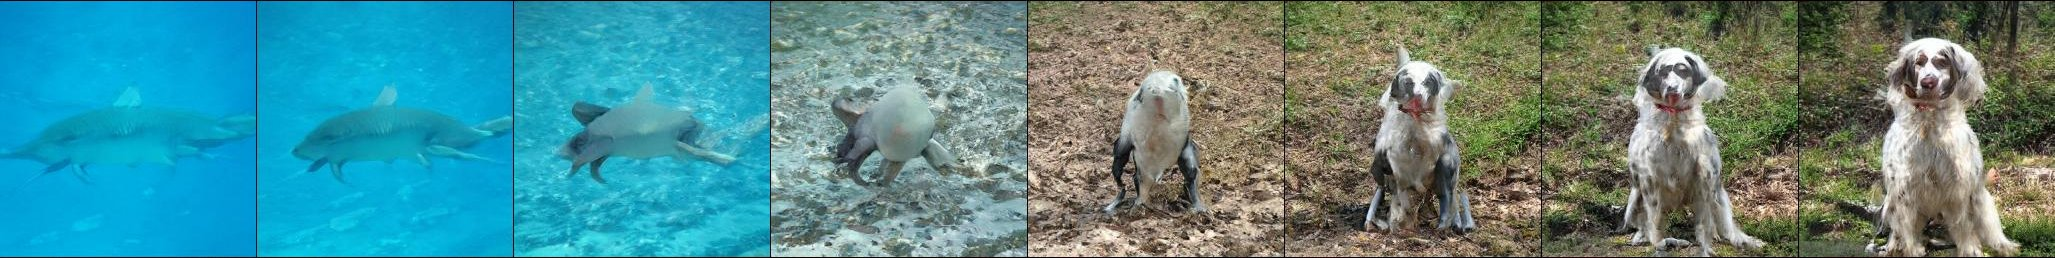
\includegraphics[width=0.98\textwidth]{images/interps0/256ZCInterp2.jpg} \\
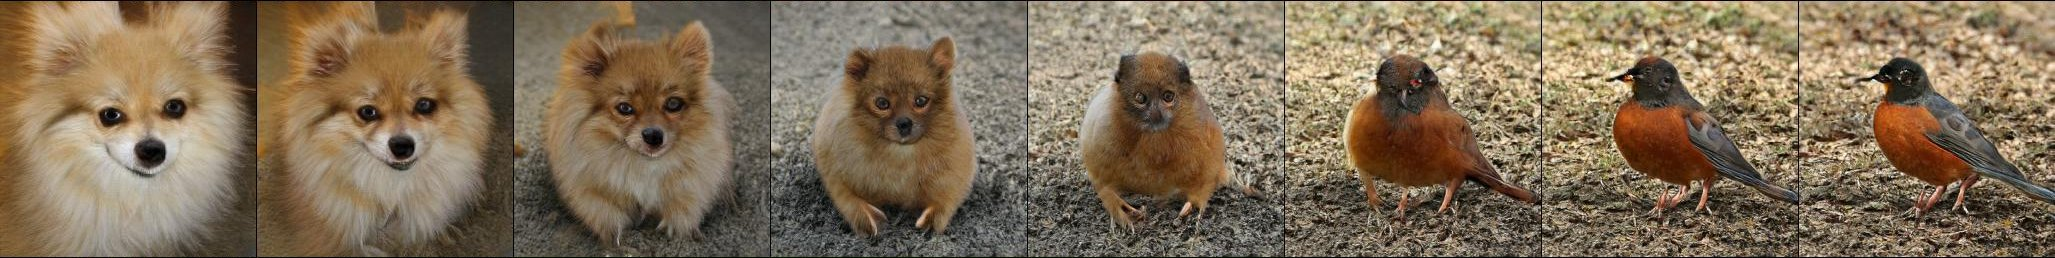
\includegraphics[width=0.98\textwidth]{images/interps0/256ZCInterp4.jpg} \\
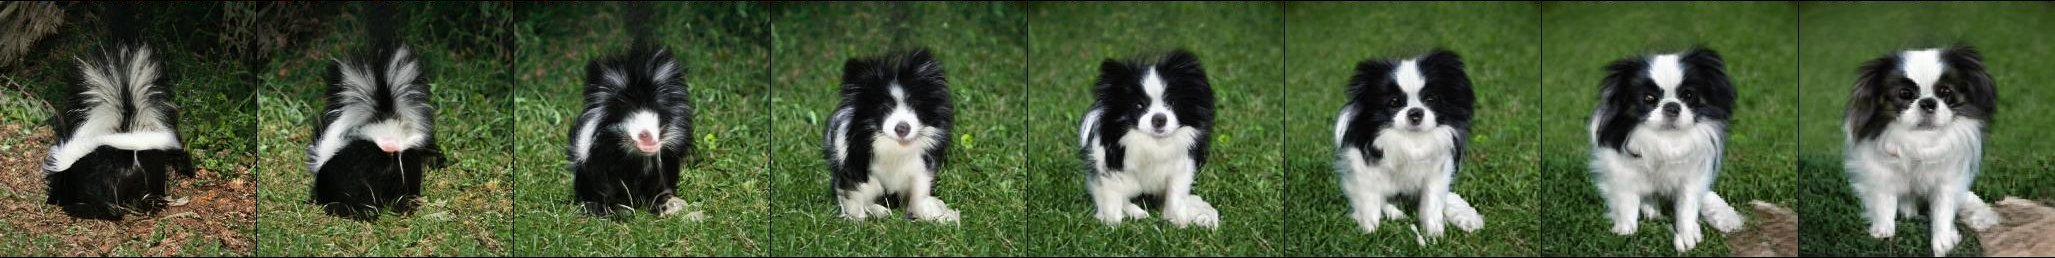
\includegraphics[width=0.98\textwidth]{images/interps0/256ZCInterp6.jpg} \\
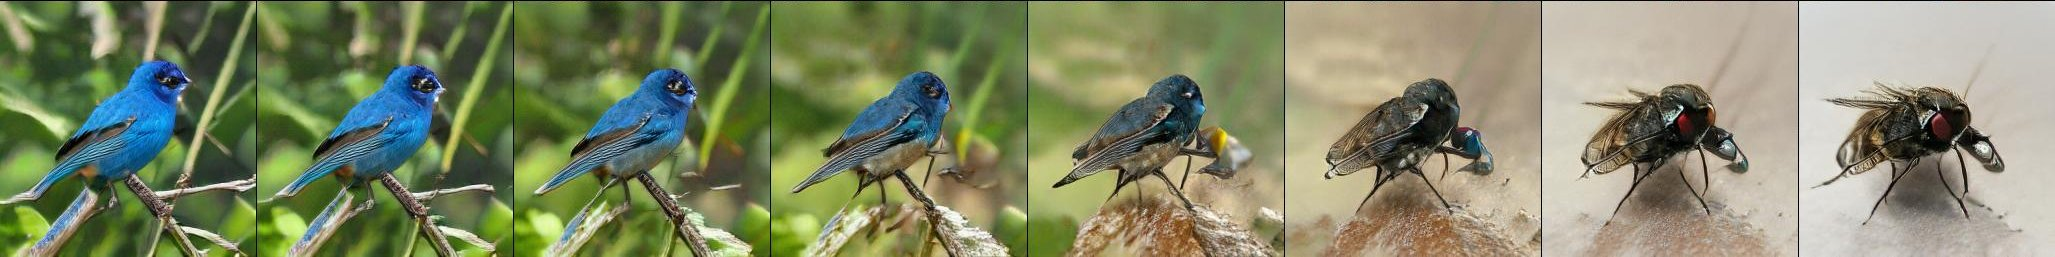
\includegraphics[width=0.98\textwidth]{images/interps0/256ZCInterp9.jpg} \\
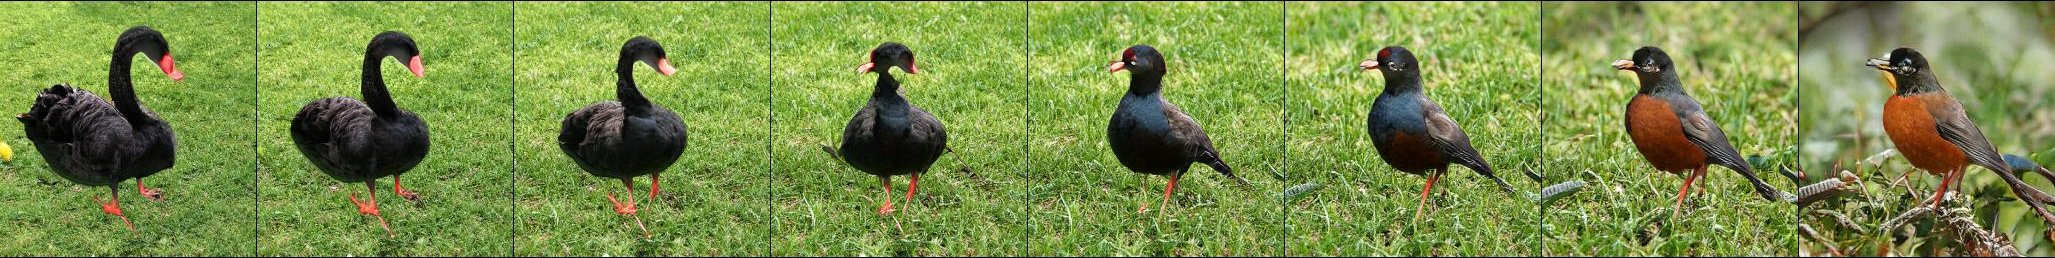
\includegraphics[width=0.98\textwidth]{images/interps0/256ZCInterp0.jpg}
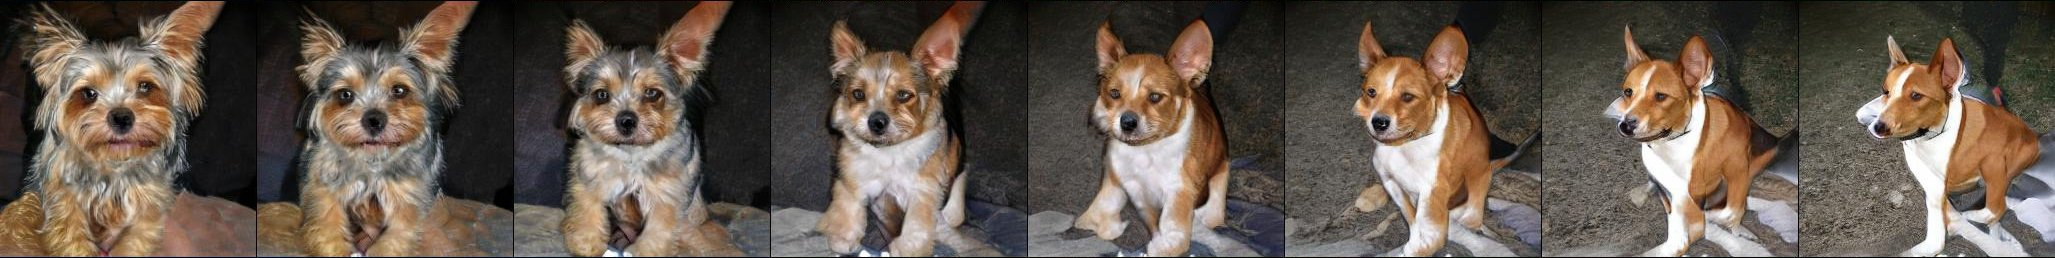
\includegraphics[width=0.98\textwidth]{images/interps0/256ZCInterp8.jpg} 
\caption{Interpolations between $z,c$ pairs.}
\label{appendix_ZCinterp}
\end{figure}

\begin{figure}[htbp]
\centering
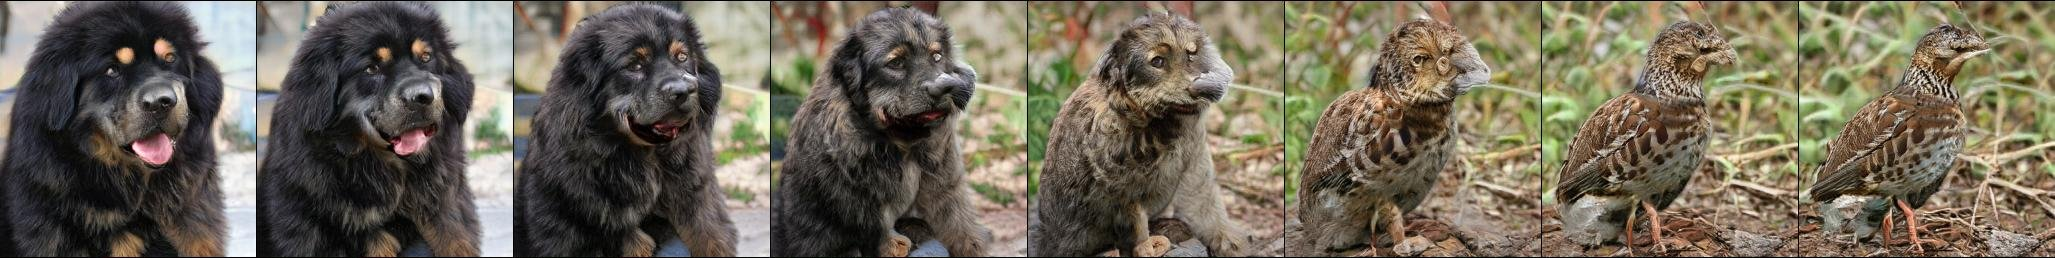
\includegraphics[width=0.98\textwidth]{images/interps0/256CInterp3.jpg} \\
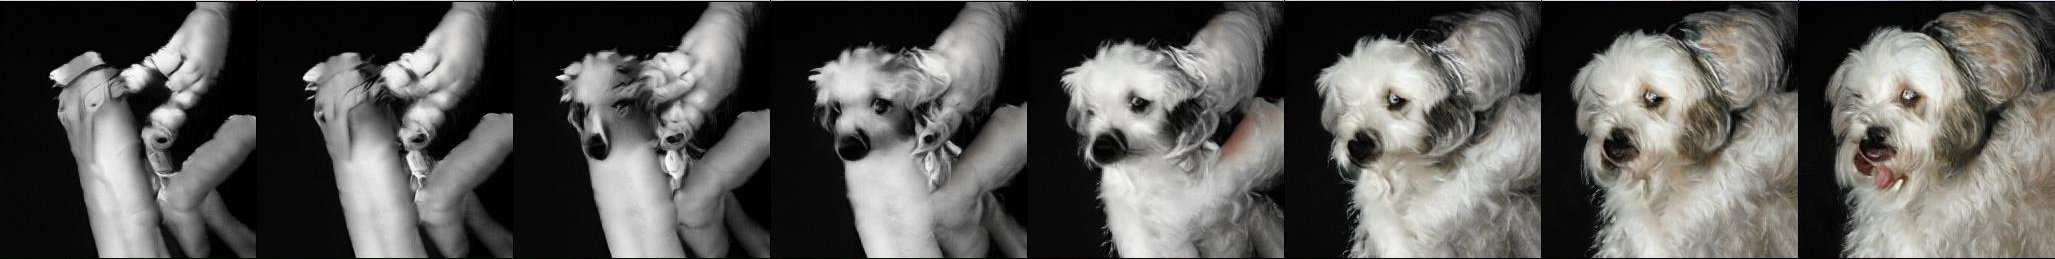
\includegraphics[width=0.98\textwidth]{images/interps0/256CInterp1.jpg} \\
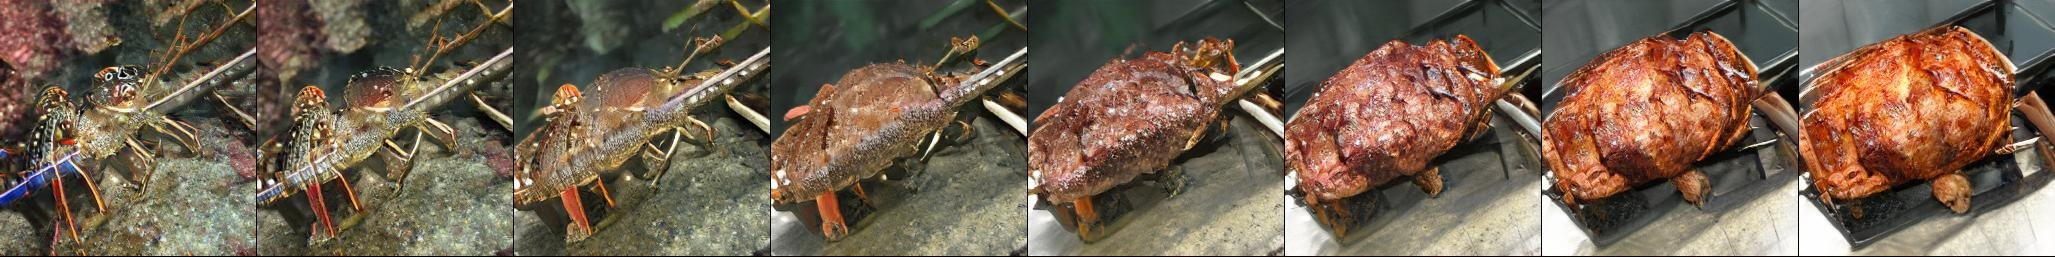
\includegraphics[width=0.98\textwidth]{images/interps0/256CInterp2.jpg} \\
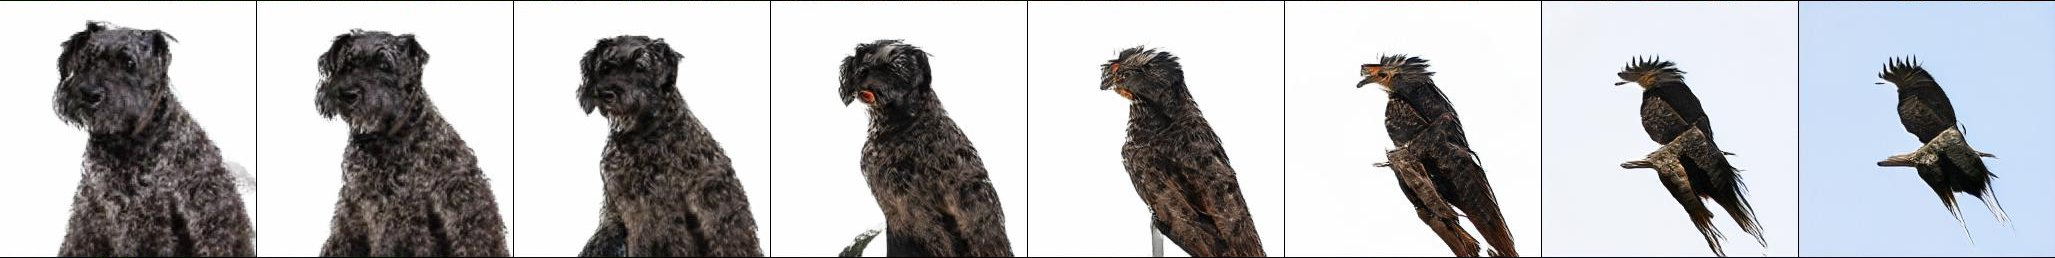
\includegraphics[width=0.98\textwidth]{images/interps0/256CInterp6.jpg} \\
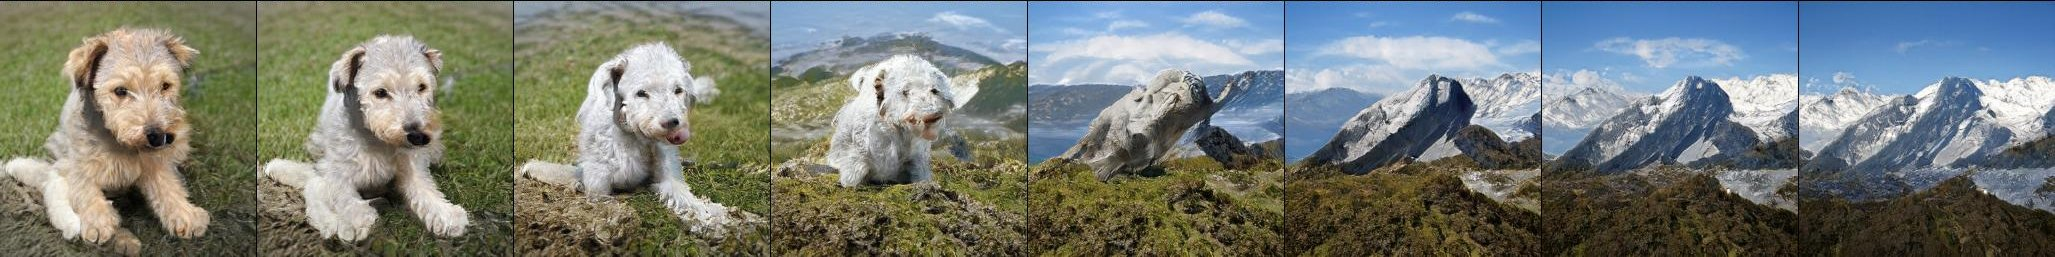
\includegraphics[width=0.98\textwidth]{images/interps0/256CInterp1a.jpg} \\
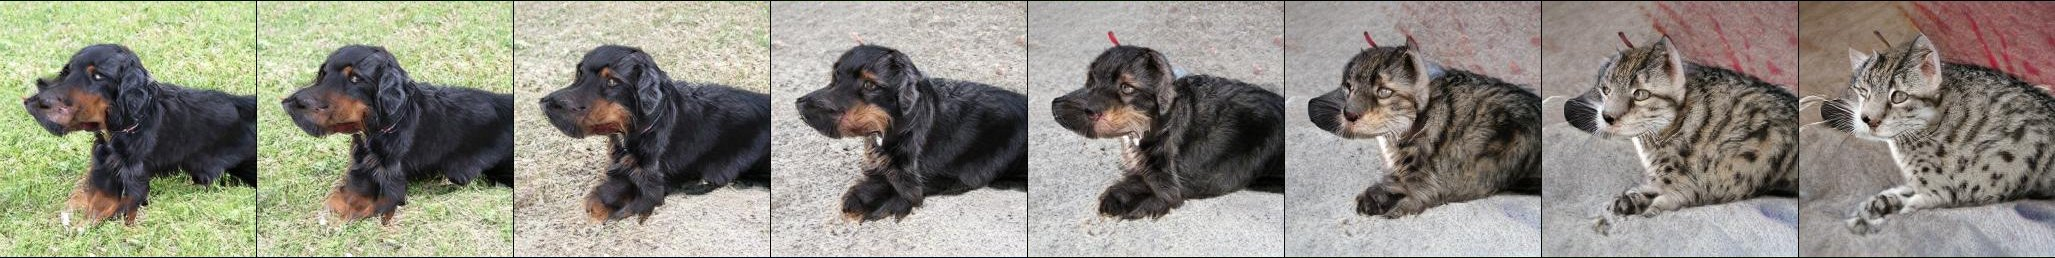
\includegraphics[width=0.98\textwidth]{images/interps0/256Cinterp7.jpg} 
\caption{Interpolations between $c$ with $z$ held constant. Pose semantics are frequently maintained between endpoints (particularly in the final row). Row 2 demonstrates that grayscale is encoded in the joint $z,c$ space, rather than in $z$.}
\label{appendix_Cinterp}
\end{figure}



\begin{figure}[htbp]
\centering
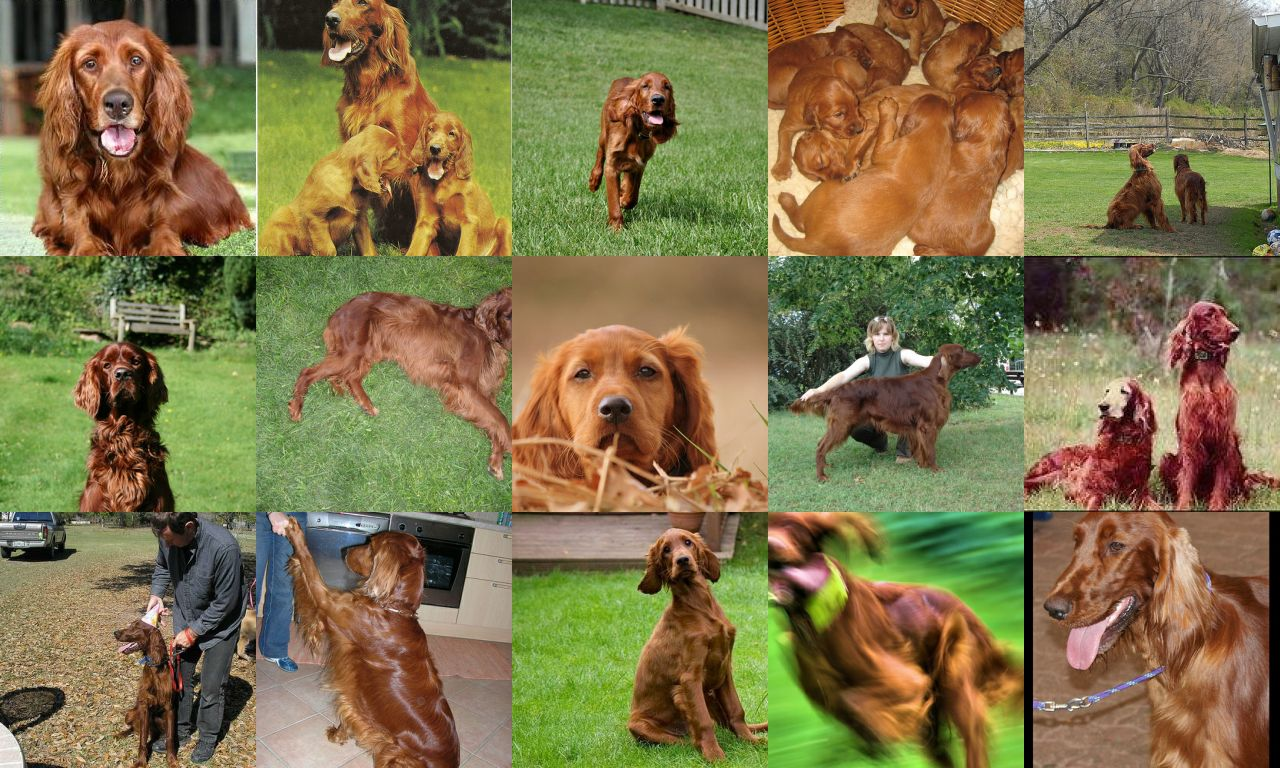
\includegraphics[width=0.98\textwidth]{images/neighbors/dog_vgg_fc7.jpg}
\caption{Nearest neighbors in VGG-16-fc7~\citep{simonyan15very} feature space. The generated image is in the top left.}
\label{appendix_nearest_dogVGG}
\end{figure}

\begin{figure}[htbp]
\centering
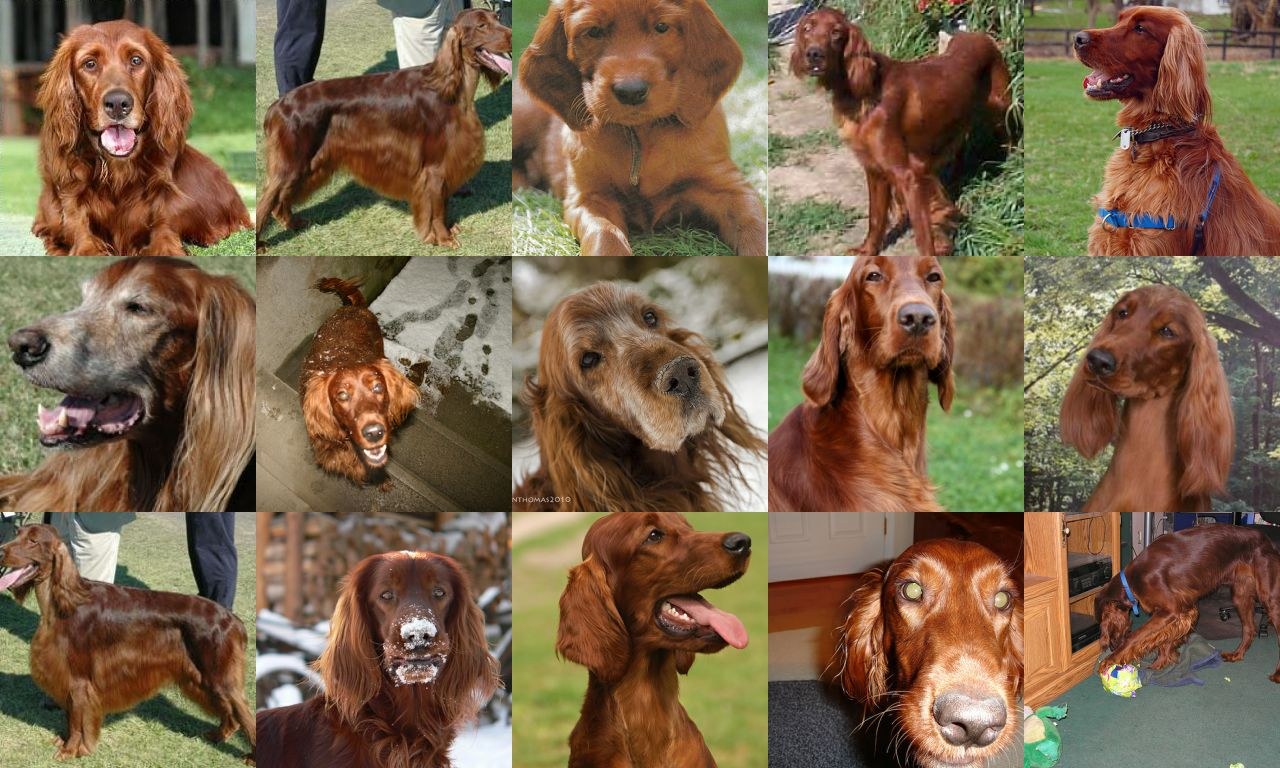
\includegraphics[width=0.98\textwidth]{images/neighbors/dog_resnet_flat.jpg}
\caption{Nearest neighbors in ResNet-50-avgpool~\citep{he2016resnets} feature space. The generated image is in the top left.}
\label{appendix_nearest_dogResNet}
\end{figure}


\begin{figure}[htbp]
\centering
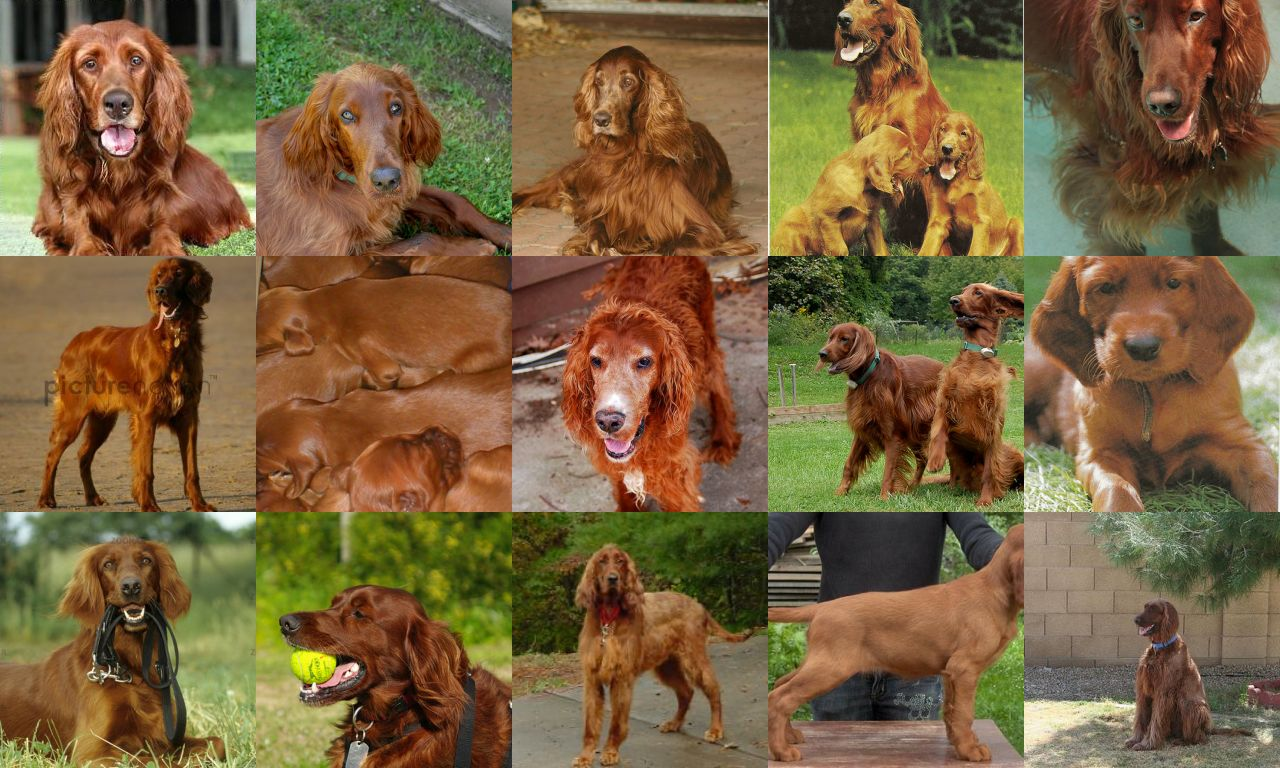
\includegraphics[width=0.98\textwidth]{images/neighbors/dog_pixel.jpg}
\caption{Nearest neighbors in pixel space. The generated image is in the top left.}
\label{appendix_nearest_dogPixel}
\end{figure}

\begin{figure}[htbp]
\centering
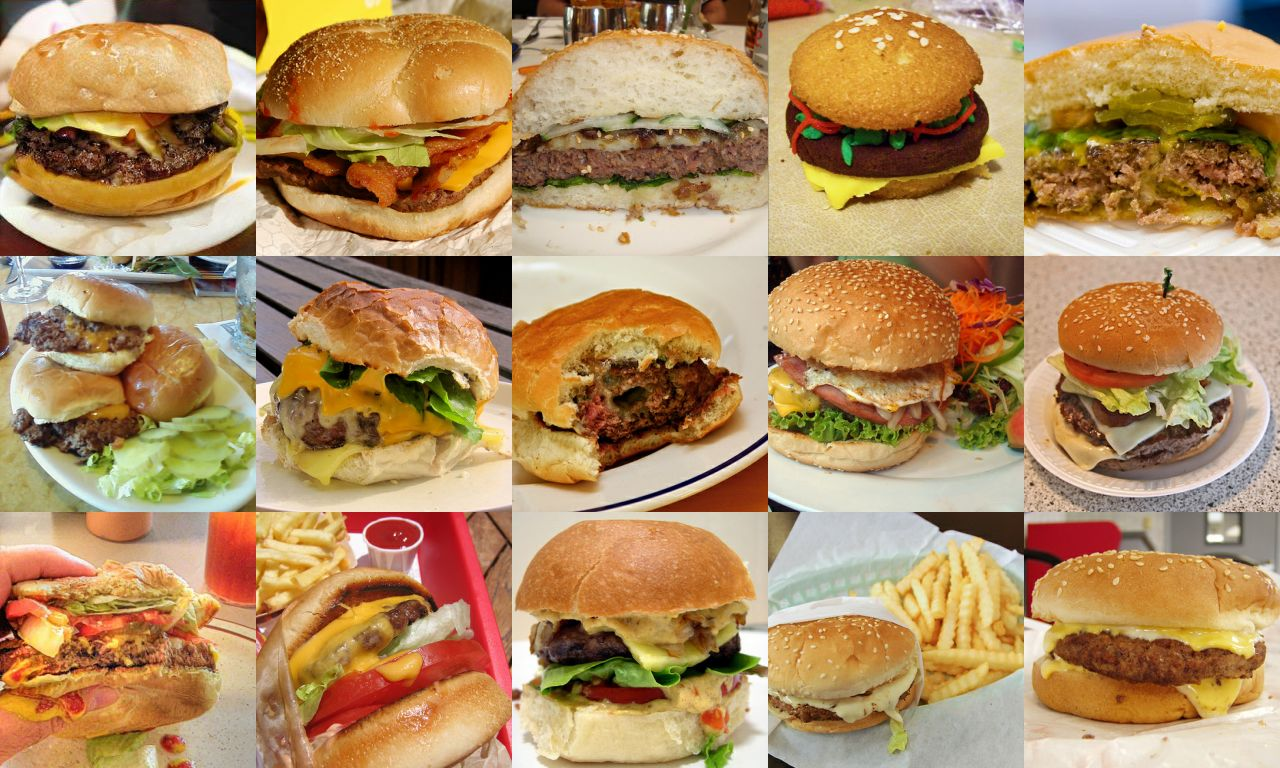
\includegraphics[width=0.98\textwidth]{images/neighbors/burger_vgg_fc7.jpg} 
\caption{Nearest neighbors in VGG-16-fc7~\citep{simonyan15very} feature space. The generated image is in the top left.}
\label{appendix_nearest_burgerVGG}
\end{figure}

\begin{figure}[htbp]
\centering
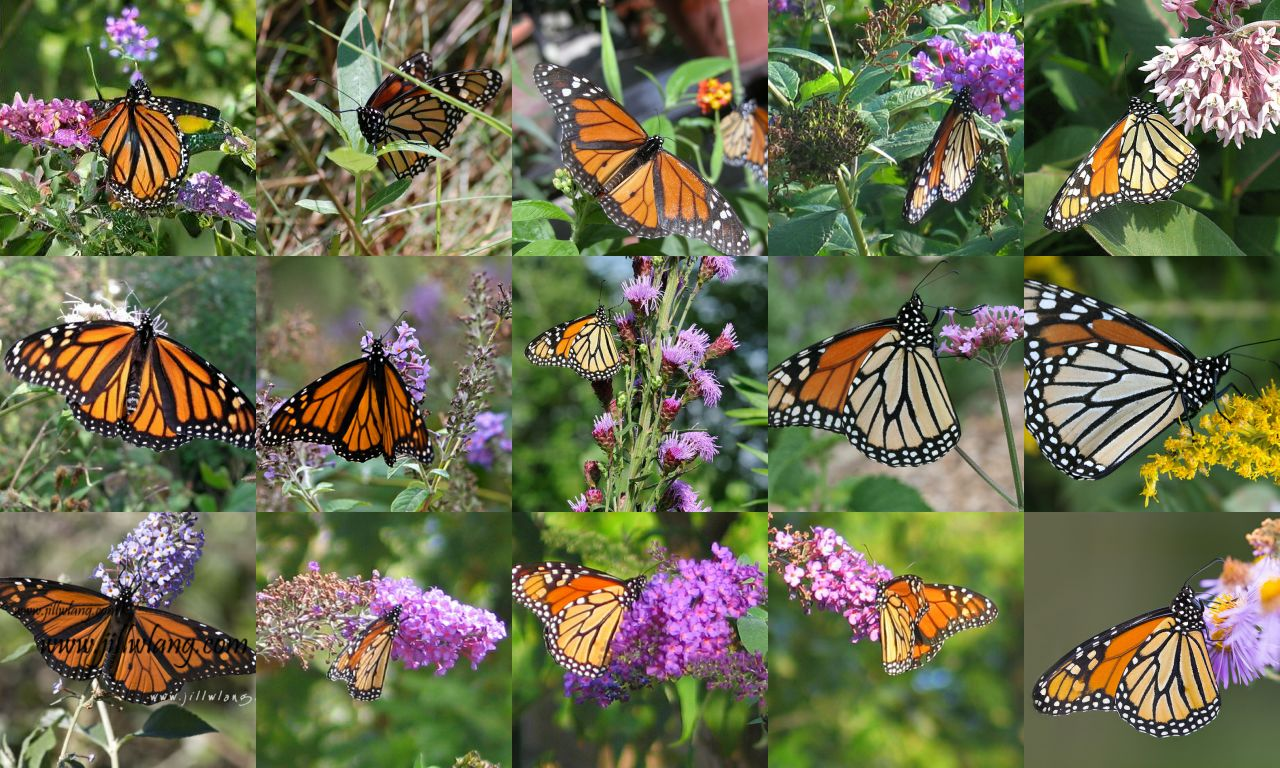
\includegraphics[width=0.98\textwidth]{images/neighbors/butterfly_resnet_flat.jpg} 
\caption{Nearest neighbors in ResNet-50-avgpool~\citep{he2016resnets} feature space. The generated image is in the top left.}
\label{appendix_nearest_MonarchResNet}
\end{figure}


\clearpage